\section{A second calculation from ignition to liner exhaustion}\label{sec:sectorcheck}
A second implementation places temperature, virgin mass and char mass at the
nodes of a moving finite-element mesh. The preceding finite-volume calculation
stores its material state at cell centres and solves for a separate surface
temperature. Both follow the same assumed heat exposure and backing properties.
The finite-element results below use the radial reduction of the sector equations,
evaluated on the Mac. Sections~\ref{sec:nativebench}--\ref{sec:coupledends} give the separate Windows MAPDL checks.

\begin{table}[H]\centering\begin{tabular}{lrrrr}\toprule
 & Finite volume & \multicolumn{3}{c}{Finite element [s]}\\
Case & 640/160 [s] & 80/20, 0.04 s & 160/40, 0.04 s & 160/40, 0.02 s \\\midrule
Sustainer Al & 110.47 & 110.58 & 110.58 & 110.53 \\
Sustainer CF & 104.25 & 104.33 & 104.23 & 104.29 \\
Booster Al & 147.61 & 147.75 & 147.74 & 147.68 \\
Booster CF & 137.95 & 138.04 & 138.03 & 137.99 \\
\bottomrule\end{tabular}\end{table}
The mesh pairs count liner and casing intervals. The solver shortens steps
at rapid reaction, fusion, front motion and output stations. In these twelve
runs, doubling the radial resolution changed the endpoint by at most 0.10 s.
Halving the time step changed it by at most 0.061 s. The largest difference
between the finest two methods was 0.073 s.

\begin{figure}[H]\centering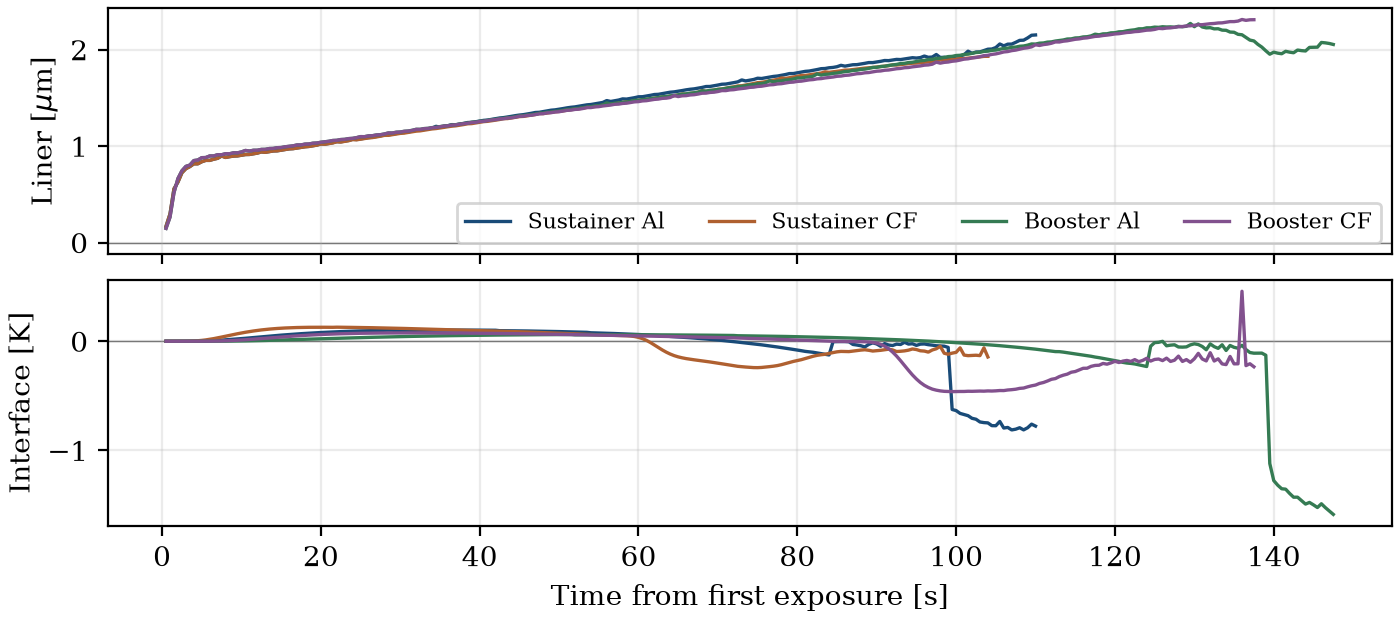
\includegraphics[width=.95\textwidth]{../analysis/sector_method_difference.png}
\caption{Finite element minus finite volume at common exposure times, sampled
every half second before either run ends. The upper panel shows remaining liner
thickness and the lower panel shows liner--casing interface temperature.}
\end{figure}
The largest sampled thickness difference is 2.3~$\mu$m and the largest
interface difference is 1.59~K. All four cases pass their baseline casing
property limits. Both aluminium walls are wholly liquid in the retained-shape
model before liner exhaustion. Both CF walls pass 1000~$^\circ$C beforehand.
An uncertainty in the imposed heat transfer affects both numerical methods
in the same direction. Their agreement gives no independent calibration of
the actual firing heat or reaction rate.
\clearpage
\section{Thermal step and recession in the moving finite-element sector}
For a radial interval with boundaries $a,b$, the row-summed linear brick
allocates volume per radian and per axial metre $(b-a)(2a+b)/6$ to its inner
node. The outer node receives the remainder of $(b^2-a^2)/2$. The equivalent
dual-volume boundary is $r_d^2=a^2+(b-a)(2a+b)/3$. These volumes carry virgin
mass $m_v$, char mass $m_c$ and sensible enthalpy $m_vh_v+m_ch_c$. At the
liner--casing interface both material contributions enter one temperature equation.
With straight sector faces of angular width $\delta$, radial conductance and the
backward-Euler transport equation are
\[
 G_e=\frac{k_e(a+b)}{2(b-a)\cos^2(\delta/2)},\qquad
 (C/\Delta t+K+H)T^*=C T^n/\Delta t+f.
\]
$C$ is the diagonal secant heat capacity from the change of sensible enthalpy
at fixed composition. It includes heat absorbed in aluminium fusion. $H$ adds
the hot and ambient film terms. The ambient coefficient includes radiation
linearized at the current iterate. $f$ includes the gas and ambient temperature
terms, prescribed incident radiation and the surface energy consumed in
forming and heating the products. The local gas film uses the previous bulk
gas flow and the current surface product flow. Its reference gas temperature
is 2504 K. $T^*$ is the transported field before local reaction.

At the exposed node the reference char kinetics are multiplied by the fraction
$m_c/(m_c+Y m_v)$, where $Y=600/1250$ is the inherited char yield. For surface
flux $j$ and starting radius $r_0$, the step ends at $r_1$ satisfying
\[
 \int_{r_0}^{r_1}(\rho_c+Y\rho_v)\,r\,dr
   = \Delta t\,j\,\frac{r_0+r_1}{2\cos(\delta/2)} .
\]
Swept virgin material releases gas and supplies its char yield for consumption.
The surface ledger includes the sensible enthalpy swept out, the sensible
enthalpy of the exiting products, the heat of pyrolysis and the effective
char-removal cost. The retained mass and sensible enthalpy are distributed
over overlapping dual volumes. The code solves the temperature from enthalpy
again after bulk pyrolysis and after equilibration at the shared interface.
The time step is shortened to the instant the remaining convertible mass
reaches zero. Restarting each short verification path reproduced its complete
terminal state and ledgers. The largest cumulative energy discrepancy in the
twelve full exposures was below $10^{-7}$ of incident film heat.

The prepared native implementation uses SOLID278 for conduction and MASS71
for the nodal thermal capacity beyond the solid element's unit volumetric
capacity. The radial predictor sets material coefficients. MAPDL must then solve
the temperatures of all sector nodes with the hot and backing faces free. The
controller checks the returned field before updating chemistry or moving the
surface. The first two short native jobs test this exchange and the saved
fields before a whole exposure can be accepted.

An independent three-dimensional assembly on Windows parsed the actual generated
elements, nodal capacities, initial conditions and surface loads. Eight Gauss
points per brick integrated heat capacity and conduction. In addition to
ignition, the checks cover the first cell merge, aluminium fusion or CF above
1000~$^\circ$C, and the final live increment for each motor. The largest
temperature difference from the radial reduction was below $10^{-9}$ K.
These checks ran in the bundled Python interpreter. Running the same input
through the native solver tests an additional software boundary.
\clearpage
